\documentclass{article}

\usepackage{amssymb,amsmath,amsthm, enumerate, graphicx}
\graphicspath{{Pictures/}}
\usepackage{lipsum}
\usepackage{float} % Allows putting an [H] in \begin{figure} to specify the exact location of %the figure
\usepackage{wrapfig} % Allows in-line images such as the example fish picture
\usepackage[top=.20in]{geometry}
\usepackage[pdftitle = {Cal Poly CSC 305}, pdfauthor = {Scott Rizzo}, pdfsubject = {Lab 7: One Night in Bangkok}, colorlinks = true, urlcolor = blue]{hyperref}

\title{Lab 07 Design}
\author{Scott Rizzo}
\date{\today}

\begin{document}
\maketitle

\section{Class Diagram}
\begin{figure}[H]
\center{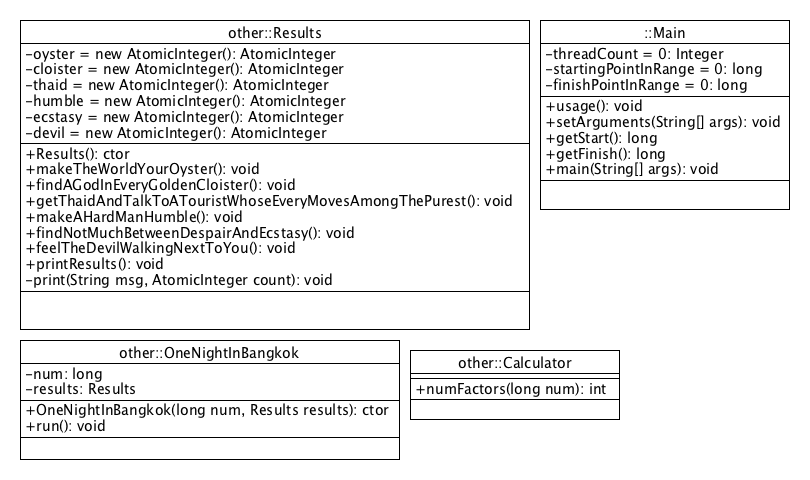
\includegraphics[width=0.9\linewidth]{lab07ClassDiagram}}
\caption{Class Diagram}
\label{fig:Hollow Star}
\end{figure}

\section{Class Responsibilities}
\subsection{Calculator}
The \texttt{Calculator} is responsible for calculating the number of factors of a given number.

\subsection{Result}
\texttt{Result} is responsible for incrementing specific AtomicInteger variables whenever certain methods are invoked.

\subsection{OneNightInBangkok}
The \texttt{OneNightInBangkok} is responsible for invoking certain methods in the Result class based on number of factors returned by Calculator class of a number.

\subsection{Main}
The \texttt{Main} class is responsible for taking command line arguments and based on those arguments run the program. In main for this lab was able to stumble upon something called Executors class, and ExecutorService interface which extends Executor interface. Using a method of Executors I was able to create a thread pool with the threads given in command line arguments. While looping through the appropriate amount of values based on what was given for the range in arguments I invoke the execute method giving it the OneNightInBangkok object to add to the queue in the thread pool. By the invoking another method which says while tasks(OneNightInBangkok's) are not done keep waiting, and when they are done shutdown and print results. 

\end{document}